\documentclass{ximera}

\input{../preamble.tex}
\author{David Kish}
\license{Creative Commons Attribution-ShareAlike 4.0 International License}


\title{Definition of Quadratics}

\begin{document}
\begin{abstract}
We explore quadratic functions.
\end{abstract}
\maketitle
\section{Quadratic Graphs}
\begin{example}
      Hannah fired a toy rocket from the ground,
      which launched into the air with an initial speed of $64$ feet per second.
      The height of the rocket can be modeled by the equation $y=-16t^2+64t$,
      where $t$ is how many seconds had passed since the launch.
      To see the shape of the graph made by this equation,
      we make a table of values and plot the points.\\
$$
\begin{array}{ccc}
                t & -16t^2+64t & Point\\
\hline
                 0 &  -16(0)^2+64(0) =0 & (0,0) \\
        1& -16(1)^2+64(1) =48&(1,48) \\
          2 & -16(2)^2+64(2) =64 &(2,64)\\
3&-16(3)^2+64(3)=48 &(3,48)\\
            4 & -16(4)^2+64(4)=0  &(4,0)
    \end{array}
$$
\begin{image}
\begin{tikzpicture}
                    \begin{axis}[xmin=-2,xmax=6,ymin=-15,ymax=75,
                                ytick=,
                                minor ytick={-10,0,...,70},
                                xlabel={$t$}]
                        \addplot+[domain=0:4,-] {-16*x^2+64*x};
                        \addplot[soliddot] coordinates {(0,0)} node[above left]{$(0,0)$};
                        \addplot[soliddot] coordinates {(1,48)} node[above left]{$(1,48)$};
                        \addplot[soliddot] coordinates {(2,64)} node[above]{$(2,64)$};
                        \addplot[soliddot] coordinates {(3,48)} node[above right]{$(3,48)$};
                        \addplot[soliddot] coordinates {(4,0)} node[above right]{$(4,0)$};
                    \end{axis}
                \end{tikzpicture}
\end{image}
\end{example}


 A curve with the shape that we see in the above figure
      is called a \textbf{parabola}.
      Notice the symmetry in figure,
      how the $y$-values in rows above the middle row match those below the middle row.
      Also notice the symmetry in the shape of the graph,
      how its left side is a mirror image of its right side.

 The first feature that we will talk about is the
      direction that a parabola opens.
      All parabolas open either upward or downward.
      This parabola in the rocket example opens downward because $a$ is negative.
      That means that for large values of $t$, the $at^2$ term will be large and negative,
      and the resulting $y$-value will be low on the $y$-axis.
      So the negative leading coefficient causes the arms of the parabola to point downward.
    

 Here are some more quadratic graphs so we can see which way they open.
\begin{image}
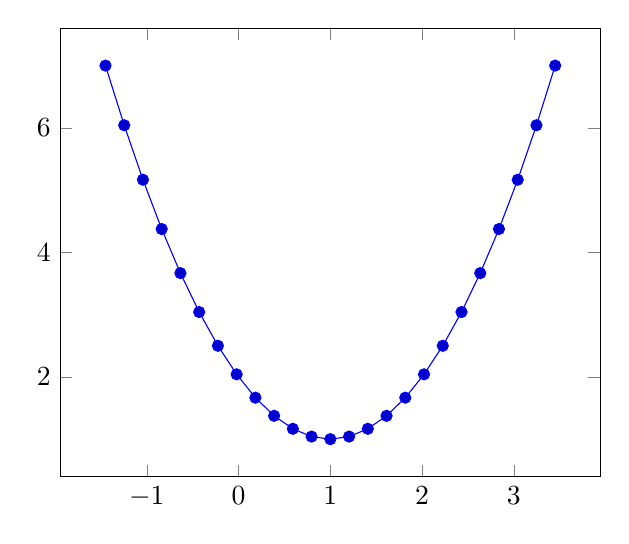
\begin{tikzpicture}
                    \begin{axis}[]
                        \addplot+[domain=-1.45:3.45] {x^2-2*x+2};
                        \end{axis}
                \end{tikzpicture}
\end{image}
\begin{image}
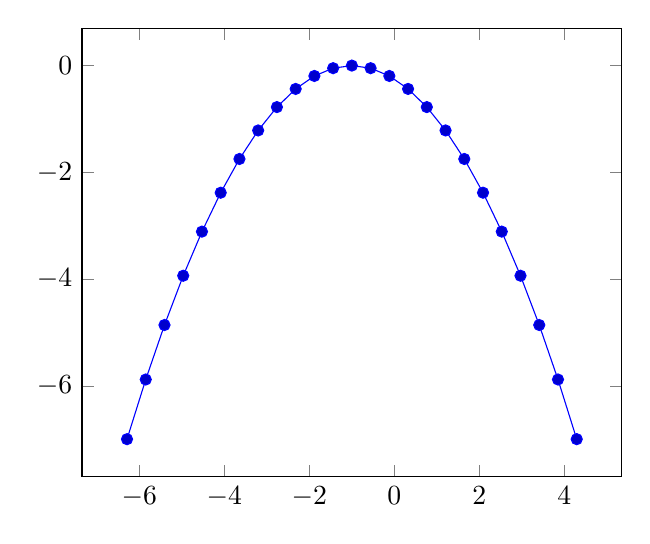
\begin{tikzpicture}
                    \begin{axis}[]
                        \addplot+[domain=-6.29:4.29] {-1/4*x^2-1/2*x-1/4};
                    \end{axis}
                \end{tikzpicture}
\end{image}
\begin{image}
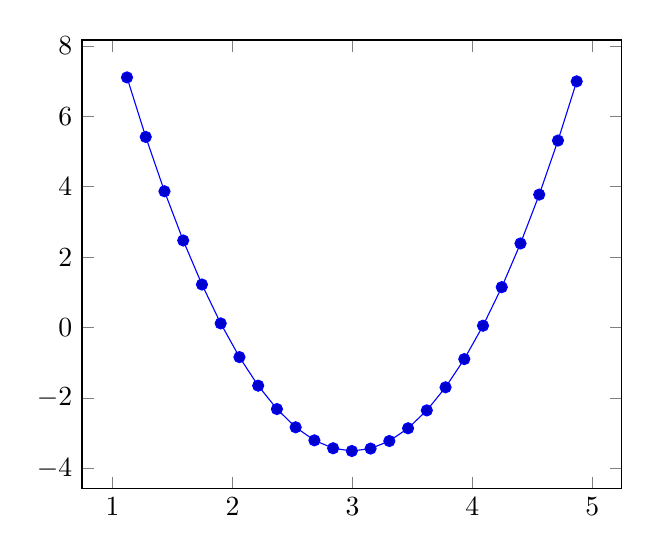
\begin{tikzpicture}
                    \begin{axis}[]
                        \addplot+[domain=1.12:4.87] {3*x^2-18*x+23.5};
                    \end{axis}
                \end{tikzpicture}
\end{image}
  The graph of a quadratic equation $y=ax^2+bx+c$ is a parabola which opens upward or downward
        according to the sign of the leading coefficient $a$.
        If the leading coefficient is positive,
        the parabola opens upward.
        If the leading coefficient is negative,
        the parabola opens downward.

 The \textbf{vertex}
      of a parabola is the highest or lowest point on the graph,
      depending uponon whether the graph opens downward or upward.
      In Example 1, the vertex is $(2,64)$.
      This tells us that Hannah's rocket reached its maximum height of $64$ feet after $2$ seconds.
      If the parabola opens downward, as in the rocket example,
      then the $y$-value of the vertex is the \textbf{maximum} $y$-value.
      If the parabola opens upward then the $y$-value of the vertex is the \textbf{minimum} $y$-value.
      The \textbf{axis of symmetry}
      is a vertical line that passes through the vertex, cutting the parabola into two symmetric halves.
      We write the axis of symmetry as an equation of a vertical line so it always starts with ``$x=$''.
      In Example 1, the equation for the axis of symmetry is $x=2$.
  

    
      The \textbf{vertical intercept} is the point where the parabola crosses the vertical axis.
      The vertical intercept is the $y$-intercept if the vertical axis is labeled $y$.
      In Example 1,
      the point $(\firsthighlight{0},\secondhighlight{0})$ is the starting point of the rocket,
      and it is where the graph crosses the $y$-axis,
      so it is the vertical intercept.
      The $y$-value of $\secondhighlight{0}$ means the rocket was on the ground
      when the $t$-value was $\firsthighlight{0}$, which was when the rocket launched.

      The \textbf{horizontal intercept(s)}
      are the points where the parabola crosses the horizontal axis.
      They are the $x$-intercepts if the horizontal axis is labeled $x$.
      The point $(0,0)$ on the path of the rocket is also a horizontal intercept.
      The $t$-value of $0$ indicates the time when the rocket was launched from the ground.
      There is another horizontal intercept at the point $(4,0)$,
      which means the rocket came back to hit the ground after $4$ seconds.
   
      It is possible for a quadratic graph to have zero, one, or two horizontal intercepts.
      The figures below show an example of each.



      
 \begin{example}
          Use technology to graph and make a table of the quadratic function $f$ defined by
          $f(x)=2x^2+4x-3$ and find each of the key points or features.
\begin{enumerate}
                \item Find the vertex.
                \item Find the vertical intercept  (i.e. the $y$-intercept).
                       \item Find the horizontal or (i.e. the $x$-intercept(s)).
               \item  Find $f(-2)$.
      \item Solve $f(x)=3$ using the graph.
           \item Solve $f(x)\le 3$ using the graph.
        \end{enumerate}
\begin{explanation}
           The specifics of how to use any one particular technology tool vary.
            Whether you use an app, a physical calculator,
            or something else, a table and graph should look like:\\
  $$
  \begin{array}{cc}
x & f(x) \\
\hline
-2 & -3 \\
-1 & -5 \\
 0 & -3 \\
 1 &  3 \\
 2 & 13 \\
  \end{array}
  $$

\begin{image}
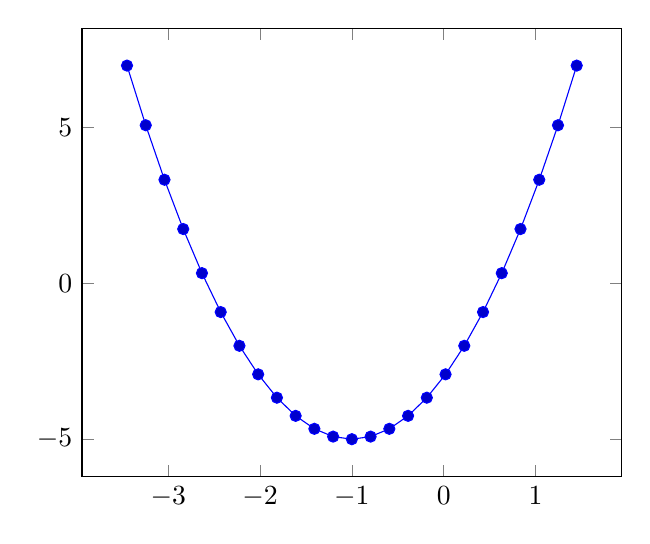
\begin{tikzpicture}
                \begin{axis}
                    \addplot+[domain=-3.449:1.449] {2*x^2+4*x-3};
                \end{axis}
            \end{tikzpicture}
\end{image}
            Additional features of your technology tool can enhance the graph to help answer these questions.
            You may be able to make the graph appear like:
\begin{image}
      \begin{tikzpicture}
                \begin{axis}[clip=false]
                    \addplot [domain=-3.449:1.449, firstcurve] {2*x^2+4*x-3} node[below right] {$y=f(x)$};
                    \addplot [domain=-7:7, secondcurve] {3} node[above left] {$y=3$};
                    \addplot [soliddot, color=thirdcolor] coordinates {(-1,-5)} node[below left] {$(-1,-5)$};
                    \addplot [soliddot, color=fourthcolor] coordinates {(1,3)} node[above right] {$(1,3)$};
                    \addplot [soliddot, color=fourthcolor] coordinates {(0,-3)} node[below right] {$(0,-3)$};
                    \addplot [soliddot, color=fourthcolor] coordinates {(-3,3)} node[above left] {$(-3,3)$};
                    \addplot [soliddot, color=fifthcolor] coordinates {(-2.581,0)} node[above left] {$(-2.6,0)$};
                    \addplot [soliddot, color=fifthcolor] coordinates {(0.581,0)} node[above right] {$(0.6,0)$};
                \end{axis}
            \end{tikzpicture}
   \end{image}
\begin{enumerate}
                \item The vertex is $(-1,-5)$.
                \item The vertical intercept is $(0,-3)$.
                \item The horizontal intercepts are approximately $(-2.6,0)$ and $(0.6,0)$.
              \item  When $x=-2$, $y=-3$, so $f(-2)=-3$.
 	 \item The solutions to $f(x)=3$ are the $x$-values where $y=3$. We graph the horizontal line $y=3$ and find the $x$-values where the graphs intersect. The solution set is $\{-3,1\}$.
       	\item  The solutions are all of the $x$-values where the function's graph is below (or touching) the line $y=3$. The interval is $[-3,1]$.
\end{enumerate}
\end{explanation}
\end{example}

A polynomal is a particular type of algebraic expression
\begin{enumerate}
\item       A company's sales, $s$
            (in millions of dollars),
            can be modeled by $2.2t+5.8$,
            where $t$ stands for the number of years since $2010$.
\item     The height of an object from the ground, $h$
            (in feet),
            launched upward from the top of a building can be modeled by $-16t^2+32t+300$,
            where $t$ represents the amount of time
            (in seconds)
            since the launch.
 \item The volume of an open-top box with a square base, $V$
            (in cubic inches),
            can be calculated by $30s^2-\frac{1}{2}s^2$,
            where $s$ stands for the length of the square base,
            and the box sides have to be cut from a certain square piece of metal.
\end{enumerate}
\section{Polynomial Vocabulary}
       A polynomial is an expression with one or more
          terms summed together.
          A term of a polynomial must either be a plain number
          or the product of a number and one or more variables raised to natural number powers.
          The expression $0$ is also considered a polynomial,
          with zero terms.
\begin{example}
Here are some examples of polynomials
\begin{enumerate}
   \item  Here are three polynomials: 
$x^2-5x+2$, $t^3-1$, $7y$.
        \item The expression $3x^4y^3+7xy^2-12xy$ is an example of a polynomial in more than one variable.
    \item   The polynomial $x^2-5x+3$ has three terms:
              $x^2$, $-5x$, and $3$.
\item The polynomial $ 3x^4+7xy^2-12xy$ also has three terms.
\item The polynomial $t^3-1$ has two terms.
\end{enumerate}
\end{example}
\begin{definition}
The coefficient
          (or numerical coefficient)
          of a term in a polynomial is the numerical factor in the term.
\end{definition}
\begin{example}
\begin{enumerate}
   \item  The coefficient of the term
              $\frac{4}{3}x^6$ is $\frac{4}{3}$.
\item   The coefficient of the second term of the polynomial $x^2-5x+3$ is $-5$.
       \item The coefficient of the term
              $\frac{y^7}{4}$ is $\frac{1}{4}$, because we can rewrite $\frac{y^7}{4}$ as $\frac{1}{4}y^7$.
\end{enumerate}
\end{example}
 A term in a polynomial with no variable factor is called a
          constant term.
\begin{example}
   The constant term of the polynomial $x^2-5x+3$ is $3$.
\end{example}
\begin{definition}
      The degree of a term is one way to measure how large it is.
          When a term only has one variable,
          its degree is the exponent on that variable.
          When a term has more than one variable,
          its degree is the sum of the exponents on the variables.
          A nonzero constant term has degree $0$.
\end{definition}
\begin{example}
  \begin{enumerate}
  \item The degree of $5x^2$ is $2$.
  \item The degree of $-\frac{4}{7}y^5$ is $5$.
  \item     The degree of $-4x^2y^3$ is $5$.
  \item  The degree of $17$ is $0$. Constant terms always have $0$ degree.
  \end{enumerate}
\end{example}

\begin{definition}
  The \dfn{degree} of a nonzero polynomial
  is the greatest degree that appears amongst its terms
\end{definition}
\begin{remark}
   To help us recognize a polynomial's degree,
        the standard convention at this level is to write a polynomial's terms in order from highest degree to lowest degree.
        When a polynomial is written in this order,
        it is written in standard form.
        For example,
        it is standard practice to write $7-4x-x^2$ as
        $-x^2-4x+7$ since $-x^2$ is the leading term.
        By writing the polynomial in standard form,
        we can look at the first term to determine both the polynomial's degree and leading term.
\end{remark}

%%%%%%%%%%
\section{Adding and Subtracting Polynomials}
        Bayani started a company that makes one product: one-gallon ketchup jugs for industrial kitchens.
        The company's production expenses only come from two things:
        supplies and labor.
        The cost of supplies, $S$
        (in thousands of dollars),
        can be modeled by $S=0.05x^2+2x+30$,
        where $x$ is number of thousands of jugs of ketchup produced.
        The labor cost for his employees, $L$
        (in thousands of dollars),
        can be modeled by $0.1x^2+4x$,
        where $x$ again represents the number of jugs they produce
        (in thousands of jugs).
        Find a model for the company's total production costs.

%%%%%%%%%%
\section{Evaluating Polynomial Expressions}

      Recall that evaluating expressions involves replacing the variable(s) in an expression with specific numbers and calculating the result.
      Here, we will look at evaluating polynomial expressions.

\begin{example}
Evaluate the expression 
\begin{center}
$-12y^3+4y^2-9y+2$ for $y=-5$ 
\end{center}
\begin{explanation}
  We will replace $y$ with $-5$ and simplify the result:
\begin{center}
$
\begin{array}{cl}
   12y^3+4y^2-9y+2 & = -12(\substitute{-5})^3+4(\substitute{-5})^2-9(\substitute{-5})+2\\
      & = -12(-125)+4(25)+45+2 \\
        & = 1647  \\
\end{array}
$
\end{center}
\end{explanation}
\end{example}

% %\section{Exponent Rules}
%   %%%%%%%%%%%%%%%%
%    \section{Product Rule}
%        If we write out $3^5\cdot 3^2$ without using exponents,
%        we'd have:
%$$
% 3^5 \cdot 3^2 = \left(3 \cdot 3\cdot 3\cdot 3\cdot 3\right) \cdot \left(3 \cdot 3\right)
%$$
%        If we then count how many $3$s are being multiplied together,
%        we find we have $5+2=7$, a total of seven $3$s.
%        So $3^5\cdot 3^2$ simplifies like this:
%       $$
%          3^5\cdot 3^2 = 3^{5+2} = 3^7
%$$
%\begin{example}          
%Simplify $x^2\cdot x^3$. \\
%\begin{explanation}       
%          To simplify $x^2\cdot x^3$,
%          we write this out in its expanded form,
%          as a product of $x$'s, we have
%$$
%            x^2\cdot x^3 =(x\cdot x)(x \cdot x \cdot x)
%            =x\cdot x\cdot x \cdot x \cdot x
%            =x^5
%   $$   
%          Note that we obtained the exponent of $5$ by adding $2$ and $3$.
%  \end{explanation}
%\end{example}
%
%      This example demonstrates our first exponent rule,
%      the Product Rule:\\
%\begin{callout}
%\textbf{ \Large Product Rule of Exponents} \\
%      When multiplying two expressions that have the same base,
%      we can simplify the product by adding the exponents.
%        $$
%x^m \cdot x^n = x^{m+n}
%$$
%\end{callout}
%   Recall that $x=x^1$. It helps to remember this when multiplying certain expressions together.
%\begin{example}        
%  Multiply $x(x^3+2)$ by using the distributive property.\\
%\begin{explanation}
%          According to the distributive property,
%        $x(x^3+2)=x\cdot x^3 + x\cdot2$
%          How can we simplify that term $x\cdot x^3$?
%          It's really the same as $x^1\cdot x^3$,
%          so according to the Product Rule, it is $x^4$.
%          So we have:
%        $$
%            x(x^3+2)=x\cdot x^3 + x\cdot2
%            =x^4+2x
%$$
%\end{explanation}
%\end{example}         
%
%%%%%%%%%%%%%%%%%
% \section{Power to a Power Rule}
%
%        If we write out $\left(3^5\right)^2$ without using exponents,
%        we'd have $3^5$ multiplied by itself:
%   $$
%         \left(3^5\right)^2 = \left(3^5\right)\cdot \left(3^5\right)
%         = \left(3\cdot 3\cdot 3\cdot 3 \cdot 3 \right) \cdot \left(3 \cdot 3\cdot 3\cdot 3\cdot 3\right)
%      $$ 
%        If we again count how many $3$s are being multiplied,
%        we have a total of two groups each with five $3$s.
%        So we'd have $2\cdot 5=10$ instances of a $3$.
%        So $\left(3^5\right)^2$ simplifies like this:
%   
%          $\left(3^5\right)^2 = 3^{2\cdot 5}$
%          $= 3^{10}$
%
%
%\begin{example}
%          Simplify $\left(x^2\right)^3$.\\
%\begin{explanation}
%          To simplify $\left(x^2\right)^3$,
%          we write this out in its expanded form,
%          as a product of $x$'s, we have
%            $\left(x^2\right)^3 =\left(x^2\right) \cdot \left(x^2\right)\cdot\left(x^2\right)$
%            $=(x \cdot x)\cdot (x \cdot x)\cdot (x \cdot x)$
%            $=x^6$
%     \end{explanation}
%          Note that we obtained the exponent of $6$ by multiplying $2$ and $3$.
%\end{example}
%      This demonstrates our second exponent rule,
%      the Power to a Power Rule:
%\begin{callout}
%\textbf{ \Large Power to a Power Rule} \\
%      when a base is raised to an exponent and that expression is raised to another exponent,
%      we multiply the exponents.
%   $$
%      \left(x^m\right)^n = x^{m \cdot n}
%   $$
%\end{callout}
%
%%%%%%%%%%%%%%%%%%%
%      \section{ Product to a Power Rule}
%        The third exponent rule deals with having multiplication inside a set of parentheses and an exponent outside the parentheses.
%        If we write out $\left(3t\right)^5$ without using an exponent,
%        we'd have $3t$ multiplied by itself five times:
%$$
%      (3t)^5= (3t)(3t)(3t)(3t)(3t)
%$$
%        Keeping in mind that there is multiplication between every $3$ and $t$,
%        and multiplication between all of the parentheses pairs,
%        we can reorder and regroup the factors:
%          $\left(3t\right)^5 = (3\cdot t)\cdot (3\cdot t)\cdot (3\cdot t)\cdot (3\cdot t)\cdot (3\cdot t)$
%          $= \left(3\cdot 3\cdot 3\cdot 3\cdot 3 \right) \cdot \left(t \cdot t \cdot t \cdot t \cdot t\right)$
%          $= 3^5 t^5$
%        We could leave it written this way if $3^5$ feels especially large.
%        But if you are able to evaluate $3^5=243$,
%        then perhaps a better final version of this expression is $243t^5$.
% 
%        We essentially applied the outer exponent to each factor inside the parentheses.
%        It is important to see how the exponent $5$ applied to \textbf{both} the $3$ \textbf{and} the $t$,
%        not just to the $t$.
%   
%
% \begin{example}   
%          Simplify $(xy)^5$.
%    
%          To simplify $(xy)^5$,
%          we write this out in its expanded form,
%          as a product of $x$'s and $y$'s, we have
%
%            $(xy)^5 =(x \cdot y) \cdot (x \cdot y) \cdot (x \cdot y) \cdot (x \cdot y) \cdot (x \cdot y)$
%            $=(x \cdot x \cdot x \cdot x \cdot x) \cdot (y \cdot y \cdot y \cdot y \cdot y)$
%            $=x^5 y^5$
%
%          Note that the exponent on $xy$ can simply be applied to both $x$ and $y$.
%\end{example}
%
%
%      This demonstrates our third exponent rule,
%      the Product to a Power Rule:
%\begin{callout}
%\textbf{ \Large Product to a Power Rule} \\
%      When a product is raised to an exponent,
%      we can apply the exponent to each factor in the product.
%$$
%        \left(x\cdot y\right)^n = x^{n}\cdot y^{n}
% $$
%\end{callout}
%
%
%%%%%%%%%%%%%%%%%%
%      \section{Summary of the Rules of Exponents for Multiplication}
%  
%
%
%          If $a$ and $b$ are real numbers,
%          and $m$ and $n$ are positive integers,
%          then we have the following rules:
% 
%\textbf{Product Rule}
%$$
%            a^{m} \cdot a^{n} = a^{m+n}
%$$
%\textbf{Power to a Power Rule}
%   $$
%           (a^{m})^{n} = a^{m\cdot n}
%   $$
% \textbf{ Product to a Power Rule}
%   $$
%           (ab)^{m} = a^{m} \cdot b^{m}
%   $$  
%      Many examples will make use of more than one exponent rule.
%      In deciding which exponent rule to work with first,
%      it's important to remember that the order of operations still applies.
%\begin{example} Simplify the following expression.
%                $\left(3^7r^5\right)^4$\\
%    \begin{explanation}
%                Since we cannot simplify anything inside the parentheses, we'll begin simplifying this expression using the Product to a Power rule.
%                We'll apply the outer exponent of 4 to each factor inside the parentheses.
%                Then we'll use the Power to a Power Rule to finish the simplification process.
%      $$          
%                  \left(3^7r^5\right)^4 = \left(3^7\right)^4 \cdot \left(r^5\right)^4
%                  = 3^{7\cdot4} \cdot r^{5\cdot 4}
%                  = 3^{28}r^{20}
%         $$      
%                Note that $3^{28}$ is too large to actually compute, even with a calculator,
%                so we leave it written as $3^{28}$.
%\end{explanation}
%\end{example}
%\begin{example}
%Simplify the following expression.
%       $\left(t^3\right)^2\cdot \left(t^4\right)^5$\\
%\begin{explanation}
%                According to the order of operations,
%                we should first simplify any exponents before carrying out any multiplication.
%                Therefore, we'll begin simplifying this by applying the Power to a Power Rule and then finish using the Product Rule.
%           $$
%                  \left(t^3\right)^2\cdot \left(t^4\right)^5 = t^{3\cdot2}\cdot t^{4\cdot5}
%                  = t^6 \cdot t^{20}
%                  = t^{6+20}
%                  = t^{26}
%$$
%\end{explanation}
%\end{example}
% \begin{remark} 
%        We cannot simplify an expression like $x^2y^3$ using the Product Rule,
%        as the factors $x^2$ and $y^3$ do not have the same base.
%\end{remark}



\end{document}
